%! TEX program = luatex
\documentclass[12pt]{article}
\usepackage{textcomp}
\usepackage{graphicx,wasysym, mdframed,xcolor,gensymb,verbatim}
\usepackage{color}
\usepackage{floatflt}

\usepackage[italian]{babel}
%%se si usa pdflatex:
%\usepackage[utf8]{inputenc}
%\usepackage[scaled=0.9]{FiraSans}
%
%i seguenti comandi funzionano con lualatex (si possono usare tutti i font di sistema come in vim o nel terminale!)
\usepackage{fontspec}
%\setmonofont{Inconsolatazi4}
%
% 0 OfficeCodePro 1=inconsolata 2=Hack
\ifcase 0 %font 0
\setmonofont[Scale=0.7,
  ItalicFont=OfficeCodePro-RegularItalic,
  BoldFont=OfficeCodePro-Bold,
  BoldItalicFont=OfficeCodePro-BoldItalic,
  UprightFont=OfficeCodePro-Regular]
  {OfficeCodePro}
\or% font 1
\setmonofont[Scale=0.7,
  ItalicFont=inconsolatalgcitalic,
  BoldFont=inconsolatalgcbold,
  BoldItalicFont=inconsolatalgcitalic,
  UprightFont=inconsolatalgc]
  {inconsolatagc}
\else% else
%
%imposto il font per listings (si possono anche indicare le varianti, i.e. italic, bold, bolditalic)
\setmonofont[Scale=0.7,
  ItalicFont=Hack-Italic,
  BoldFont=Hack-Bold,
  BoldItalicFont=Hack-BoldItalic,
  UprightFont=Hack-Regular]
  {Hack}
\fi
%
\usepackage[T1]{fontenc}
% un'alternativa a listingsutf8 è il pacchetto minted ma richiede una libreria python chiamata Pygments
\usepackage{listingsutf8}
\definecolor{verdeoliva}{rgb}{0.3,0.3,0}
\definecolor{grigio}{rgb}{0.5,0.5,0.5}
\definecolor{blumarino}{rgb}{0.0,0,0.5}
\definecolor{panna}{rgb}{0.98,0.98,0.94}
\def\lstlistingname{Listato}
\lstset{%
  %inputencoding=utf8,
  breaklines=true,
  %extendedchars=true,              % lets you use non-ASCII characters; for 8-bits encodings only, does not work with UTF-8
  %literate=%
  %       {á}{{\'a}}1
  %       {í}{{\'i}}1
  %       {é}{{\'e}}1
  %       {ý}{{\'y}}1
  %       {ú}{{\'u}}1
  %       {ó}{{\'o}}1,
  backgroundcolor=\color{panna},   % choose the background color; you must add \usepackage{color} or \usepackage{xcolor}; should come as last argument
% basicstyle=\footnotesize\ttfamily,
  basicstyle=\ttfamily,            % è selezionato all'inizio di ogni listing
  belowskip=-0.2\baselineskip,
% basicstyle=\footnotesize,        % the size of the fonts that are used for the code
  breakatwhitespace=false,         % sets if automatic breaks should only happen at whitespace
% breaklines=true,                 % sets automatic line breaking
  captionpos=b,                    % sets the caption-position to bottom
  commentstyle=\itshape\color{verdeoliva}, % comment style (nota: all'inizio del listing seleziona \ttfamily, perciò qui seleziona la variante italic)
% deletekeywords={},            % if you want to delete keywords from the given language
% escapeinside={\%*}{*)},          % if you want to add LaTeX within your code
% firstnumber=1000,                % start line enumeration with line 1000
  frame=single,	                   % adds a frame around the code
  keepspaces=true,                 % keeps spaces in text, useful for keeping indentation of code (possibly needs columns=flexible)
  keywordstyle=\bfseries\color{blue},       % keyword style
% language=Octave,                 % the language of the code
% morekeywords={*,},            % if you want to add more keywords to the set
  numbers=left,                    % where to put the line-numbers; possible values are (none, left, right)
  numbersep=5pt,                   % how far the line-numbers are from the code
  numberstyle=\tiny\color{grigio}, % the style that is used for the line-numbers
  rulecolor=\color{black},         % if not set, the frame-color may be changed on line-breaks within not-black text (e.g. comments (green here))
  showspaces=false,                % show spaces everywhere adding particular underscores; it overrides 'showstringspaces'
  showstringspaces=false,          % underline spaces within strings only
  showtabs=false,                  % show tabs within strings adding particular underscores
  stepnumber=1,                    % the step between two line-numbers. If it's 1, each line will be numbered
  stringstyle=\color{blumarino},   % string literal style
  tabsize=2,	                   % sets default tabsize to 2 spaces
  title=\lstname%                  % show the filename of files included with \lstinputlisting; also try caption instead of title
}



%%%%%%%%%%%%%%%%%%%%%
\usepackage{listings}
\usepackage{xcolor}
\usepackage{bm}

%New colors defined below
\definecolor{codegreen}{rgb}{0,0.6,0}
\definecolor{codegray}{rgb}{0.5,0.5,0.5}
\definecolor{codepurple}{rgb}{0.58,0,0.82}
\definecolor{backcolour}{rgb}{0.95,0.95,0.92}

%Code listing style named "mystyle"
\lstdefinestyle{mystyle}{
  backgroundcolor=\color{backcolour},   commentstyle=\color{codegreen},
  keywordstyle=\color{magenta},
  numberstyle=\tiny\color{codegray},
  stringstyle=\color{codepurple},
  basicstyle=\ttfamily\footnotesize,
  breakatwhitespace=false,         
  breaklines=true,                 
  captionpos=b,                    
  keepspaces=true,                 
  numbers=left,                    
  numbersep=5pt,                  
  showspaces=false,                
  showstringspaces=false,
  showtabs=false,                  
  tabsize=2
}
\lstset{style=mystyle}
%%%%%%%%%%%%%%%%%%%

\newcommand{\voto}[1]{[\textbf{#1} punti]}
\def\cmu{\mbox{cm$^{-1}$}}
\def\half{\frac{1}{2}}

\voffset -2cm
\hoffset -2.5cm
%\marginparwidth 0cm
\textheight 22cm
\textwidth 17cm
%\oddsidemargin  0.2cm                                                                                         
%\evensidemargin 0.4cm                                                                                         
\parindent=0pt

\begin{document}
\pagestyle{empty}

\begin{center}
{\Large \bf  Laboratorio di Calcolo per Fisici, Quarta esercitazione\\[2mm]}
{\large Canale D-K, Docente: Livia Soffi, \\Esercitatori: Prof. S. Rahatlou e Prof. R. Faccini}
\end{center}
\vspace{4mm}

\colorbox{yellow}{\begin{minipage}{17cm}
  Lo scopo della quarta esercitazione di laboratorio \`e di simulare il gioco della roulette sfruttando la \textbf{generazione di numeri pseudocasuali}.
\end{minipage}}
\vspace{2mm}
%\vspace{1mm}
%
%

\hrule
\vspace{2mm}
Nel gioco della roulette semplificato, la ruota contiene \textbf{36 caselle numerate da 1 a 36}. Il croupier lancia una piccola palla bianca, e la fa ruotare nella roulette, finché essa non si ferma su uno dei numeri. Le puntate sono piazzate sul tavolo, secondo i possibili esiti del lancio della palla. Un giocatore pu\`o scommettere che la pallina finisca su:

\begin{minipage}{10cm}
\vspace{2mm}
\begin{itemize}
\item Un \textbf{numero preciso} compreso tra 1 e 36
\item Un numero \textbf{dispari o pari}
\item Un \textbf{numero basso} [1-18] \textbf{o alto} [19-39]
\end{itemize}
 \end{minipage}
    \begin{minipage}{0.5\textwidth}
  %   \begin{figure}[h]
        \begin{center}
        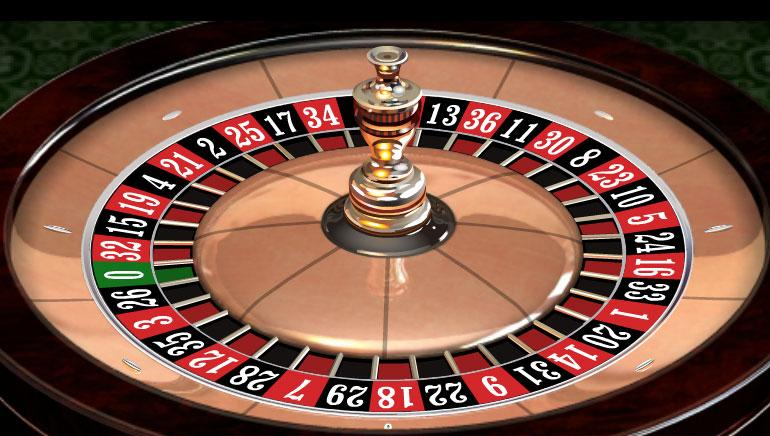
\includegraphics[scale=0.2]{roulette.jpg}
        \end{center}
   %   \end{figure}
    \end{minipage}
 \vspace{2mm}  
\hrule
\vspace{2mm}
\textbf{$\RHD$ Prima parte (obbligatoria)} 
\vspace{2mm}

Scrivere un programma chiamato \textbf{\emph{roulette.c}} che simuli $N$ lanci della pallina.
\begin{enumerate}
\item Stampare un messaggio di istruzioni per l'utente che chieda di \textbf{inserire $N$}.
\item Acquisire il numero di lanci $N$, assicurandosi che $N$ sia minore di 10000.
\item Per ogni lancio:
\begin{enumerate}
\item generare un numero \textbf{intero random tra 1 e 36}
\item Riconoscere se il numero generato \`e pari ($P$) o dispari ($D$), alto ($A$) o basso ($B$).
\item Stampare su schermo l'esito del lancio nel formato dell'esempio:\\ \emph{"Hai generato il numero 7. Il numero e' dispari e basso."} 
\item Contare quante volte si verificano ciascuno dei casi precedenti:$P/D/A/B$
\end{enumerate}
\item Alla fine degli $N$ lanci stampare \textbf{la frequenza con cui si e' verificato ciascun risultato $P/D/A/B$}.
\item Eseguire il programma \emph{roulette.c} per $N=10,100, 1000, 10000$. \item Scrivere su un file \emph{esiti.dat} il valore di $N$ e delle frequenze con cui si sono verificati i risultati $P/D/A/B$. Come cambiano le frequenze in funzione di N? Il risultato \`e coerente con le vostre aspettative?
\end{enumerate}
\colorbox{yellow}{\begin{minipage}{17cm}
NB. Si ricorda che per compilare ed eseguire il programma in C si deve digitare sul terminale:\\
\textbf{gcc roulette.c -o roulette.x -lm -Wall \\
./roulette.x}
\end{minipage}}


\newpage
\hrule
\vspace{2mm}
\textbf{$\RHD$ Seconda parte (facoltativa)} 
\vspace{2mm}

Scrivere  il programma \textbf{\emph{gioco.c}} per simulare una vera partita di roulette. 

\begin{enumerate}

\item All'inizio del gioco il giocatore ha un \textbf{credito di 100 euro} 

\item Chiedere all'utente \textbf{che somma vuole puntare}. La cifra deve essere compresa tra 2 e 10 euro e comunque sempre inferiore o uguale al credito. 

\item Chiedere all'utente \textbf{su che numero scommette}. Controllare che il numero sia tra 1 e 36.

\item Generare il numero random tra 1 e 36 corrispondente all'esito del lancio della pallina

\item Se la pallina \`e finita sullo stesso numero scelto dall'utente, questi \textbf{vince due volte la sua posta, altrimenti perde la posta}.

\item Stampare su schermo il numero uscito e un messaggio che dica all'utente \textbf{se ha vinto o se ha perso e a quanto ammonta il suo credito}.

\item Implementare l'opportuno costrutto iterativo che permetta all'utente di continuare a giocare \textbf{finch\`e il credito e' almeno 2 euro e comunque per non pi\`u di 20 mani}.

\item Scrivere un messaggio che informi l'utente alla fine del gioco. Specificare quante mani sono state giocate e se il suo credito finale \`e nullo, altrimenti stamparne il valore.
\end{enumerate}
\vspace{2cm}

\colorbox{yellow}{\begin{minipage}{17cm}

\textbf{Suggerimenti:}
\begin{itemize}
\item La funzione \textbf{rand()} definita nella libreria \textbf{stdlib.h} permette di generare numeri \textbf{interi tra 0 e RAND\_MAX}.
\item L'algoritmo di generazione deve essere inizializzato con un seme \textbf{una sola volta}:\\
\textbf{int seed;\\
seed  = time(0);\\
srand(seed);}
\item Per generare un numero \textbf{intero} casuale compreso \textbf{tra 1 e nmax} si usa la proprietà della funzione modulo (\%):\\
\textbf{i=rand() \% nmax + 1;}
\item Nel calcolo della frequenza, prima di fare il rapporto di due interi bisogna fare il casting del numeratore a double come segue:\\
\textbf{double freq};\\
\textbf{freq = (double)Num/Den;}

\end{itemize}
\end{minipage}}


\vspace{2mm}


\end{document}


\begin{lstlisting}[language=C]

\end{lstlisting}
